\documentclass{ximera}

%\usepackage{todonotes}

\newcommand{\todo}{}

\usepackage{esint} % for \oiint
\ifxake%%https://math.meta.stackexchange.com/questions/9973/how-do-you-render-a-closed-surface-double-integral
\renewcommand{\oiint}{{\large\bigcirc}\kern-1.56em\iint}
\fi


\graphicspath{
  {./}
  {ximeraTutorial/}
  {basicPhilosophy/}
  {functionsOfSeveralVariables/}
  {normalVectors/}
  {lagrangeMultipliers/}
  {vectorFields/}
  {greensTheorem/}
  {shapeOfThingsToCome/}
  {dotProducts/}
  {partialDerivativesAndTheGradientVector/}
  {../productAndQuotientRules/exercises/}
  {../normalVectors/exercisesParametricPlots/}
  {../continuityOfFunctionsOfSeveralVariables/exercises/}
  {../partialDerivativesAndTheGradientVector/exercises/}
  {../directionalDerivativeAndChainRule/exercises/}
  {../commonCoordinates/exercisesCylindricalCoordinates/}
  {../commonCoordinates/exercisesSphericalCoordinates/}
  {../greensTheorem/exercisesCurlAndLineIntegrals/}
  {../greensTheorem/exercisesDivergenceAndLineIntegrals/}
  {../shapeOfThingsToCome/exercisesDivergenceTheorem/}
  {../greensTheorem/}
  {../shapeOfThingsToCome/}
  {../separableDifferentialEquations/exercises/}
  {vectorFields/}
}

\newcommand{\mooculus}{\textsf{\textbf{MOOC}\textnormal{\textsf{ULUS}}}}

\usepackage{tkz-euclide}
\usepackage{tikz}
\usepackage{tikz-cd}
\usetikzlibrary{arrows}
\tikzset{>=stealth,commutative diagrams/.cd,
  arrow style=tikz,diagrams={>=stealth}} %% cool arrow head
\tikzset{shorten <>/.style={ shorten >=#1, shorten <=#1 } } %% allows shorter vectors

\usetikzlibrary{backgrounds} %% for boxes around graphs
\usetikzlibrary{shapes,positioning}  %% Clouds and stars
\usetikzlibrary{matrix} %% for matrix
\usepgfplotslibrary{polar} %% for polar plots
\usepgfplotslibrary{fillbetween} %% to shade area between curves in TikZ
%\usetkzobj{all}
\usepackage[makeroom]{cancel} %% for strike outs
%\usepackage{mathtools} %% for pretty underbrace % Breaks Ximera
%\usepackage{multicol}
\usepackage{pgffor} %% required for integral for loops



%% http://tex.stackexchange.com/questions/66490/drawing-a-tikz-arc-specifying-the-center
%% Draws beach ball
\tikzset{pics/carc/.style args={#1:#2:#3}{code={\draw[pic actions] (#1:#3) arc(#1:#2:#3);}}}



\usepackage{array}
\setlength{\extrarowheight}{+.1cm}
\newdimen\digitwidth
\settowidth\digitwidth{9}
\def\divrule#1#2{
\noalign{\moveright#1\digitwidth
\vbox{\hrule width#2\digitwidth}}}




% \newcommand{\RR}{\mathbb R}
% \newcommand{\R}{\mathbb R}
% \newcommand{\N}{\mathbb N}
% \newcommand{\Z}{\mathbb Z}

\newcommand{\sagemath}{\textsf{SageMath}}


%\renewcommand{\d}{\,d\!}
%\renewcommand{\d}{\mathop{}\!d}
%\newcommand{\dd}[2][]{\frac{\d #1}{\d #2}}
%\newcommand{\pp}[2][]{\frac{\partial #1}{\partial #2}}
% \renewcommand{\l}{\ell}
%\newcommand{\ddx}{\frac{d}{\d x}}

% \newcommand{\zeroOverZero}{\ensuremath{\boldsymbol{\tfrac{0}{0}}}}
%\newcommand{\inftyOverInfty}{\ensuremath{\boldsymbol{\tfrac{\infty}{\infty}}}}
%\newcommand{\zeroOverInfty}{\ensuremath{\boldsymbol{\tfrac{0}{\infty}}}}
%\newcommand{\zeroTimesInfty}{\ensuremath{\small\boldsymbol{0\cdot \infty}}}
%\newcommand{\inftyMinusInfty}{\ensuremath{\small\boldsymbol{\infty - \infty}}}
%\newcommand{\oneToInfty}{\ensuremath{\boldsymbol{1^\infty}}}
%\newcommand{\zeroToZero}{\ensuremath{\boldsymbol{0^0}}}
%\newcommand{\inftyToZero}{\ensuremath{\boldsymbol{\infty^0}}}



% \newcommand{\numOverZero}{\ensuremath{\boldsymbol{\tfrac{\#}{0}}}}
% \newcommand{\dfn}{\textbf}
% \newcommand{\unit}{\,\mathrm}
% \newcommand{\unit}{\mathop{}\!\mathrm}
% \newcommand{\eval}[1]{\bigg[ #1 \bigg]}
% \newcommand{\seq}[1]{\left( #1 \right)}
% \renewcommand{\epsilon}{\varepsilon}
% \renewcommand{\phi}{\varphi}


% \renewcommand{\iff}{\Leftrightarrow}

% \DeclareMathOperator{\arccot}{arccot}
% \DeclareMathOperator{\arcsec}{arcsec}
% \DeclareMathOperator{\arccsc}{arccsc}
% \DeclareMathOperator{\si}{Si}
% \DeclareMathOperator{\scal}{scal}
% \DeclareMathOperator{\sign}{sign}


%% \newcommand{\tightoverset}[2]{% for arrow vec
%%   \mathop{#2}\limits^{\vbox to -.5ex{\kern-0.75ex\hbox{$#1$}\vss}}}
% \newcommand{\arrowvec}[1]{{\overset{\rightharpoonup}{#1}}}
% \renewcommand{\vec}[1]{\arrowvec{\mathbf{#1}}}
% \renewcommand{\vec}[1]{{\overset{\boldsymbol{\rightharpoonup}}{\mathbf{#1}}}}

% \newcommand{\point}[1]{\left(#1\right)} %this allows \vector{ to be changed to \vector{ with a quick find and replace
% \newcommand{\pt}[1]{\mathbf{#1}} %this allows \vec{ to be changed to \vec{ with a quick find and replace
% \newcommand{\Lim}[2]{\lim_{\point{#1} \to \point{#2}}} %Bart, I changed this to point since I want to use it.  It runs through both of the exercise and exerciseE files in limits section, which is why it was in each document to start with.

% \DeclareMathOperator{\proj}{\mathbf{proj}}
% \newcommand{\veci}{{\boldsymbol{\hat{\imath}}}}
% \newcommand{\vecj}{{\boldsymbol{\hat{\jmath}}}}
% \newcommand{\veck}{{\boldsymbol{\hat{k}}}}
% \newcommand{\vecl}{\vec{\boldsymbol{\l}}}
% \newcommand{\uvec}[1]{\mathbf{\hat{#1}}}
% \newcommand{\utan}{\mathbf{\hat{t}}}
% \newcommand{\unormal}{\mathbf{\hat{n}}}
% \newcommand{\ubinormal}{\mathbf{\hat{b}}}

% \newcommand{\dotp}{\bullet}
% \newcommand{\cross}{\boldsymbol\times}
% \newcommand{\grad}{\boldsymbol\nabla}
% \newcommand{\divergence}{\grad\dotp}
% \newcommand{\curl}{\grad\cross}
%\DeclareMathOperator{\divergence}{divergence}
%\DeclareMathOperator{\curl}[1]{\grad\cross #1}
% \newcommand{\lto}{\mathop{\longrightarrow\,}\limits}

% \renewcommand{\bar}{\overline}

\colorlet{textColor}{black}
\colorlet{background}{white}
\colorlet{penColor}{blue!50!black} % Color of a curve in a plot
\colorlet{penColor2}{red!50!black}% Color of a curve in a plot
\colorlet{penColor3}{red!50!blue} % Color of a curve in a plot
\colorlet{penColor4}{green!50!black} % Color of a curve in a plot
\colorlet{penColor5}{orange!80!black} % Color of a curve in a plot
\colorlet{penColor6}{yellow!70!black} % Color of a curve in a plot
\colorlet{fill1}{penColor!20} % Color of fill in a plot
\colorlet{fill2}{penColor2!20} % Color of fill in a plot
\colorlet{fillp}{fill1} % Color of positive area
\colorlet{filln}{penColor2!20} % Color of negative area
\colorlet{fill3}{penColor3!20} % Fill
\colorlet{fill4}{penColor4!20} % Fill
\colorlet{fill5}{penColor5!20} % Fill
\colorlet{gridColor}{gray!50} % Color of grid in a plot

\newcommand{\surfaceColor}{violet}
\newcommand{\surfaceColorTwo}{redyellow}
\newcommand{\sliceColor}{greenyellow}




\pgfmathdeclarefunction{gauss}{2}{% gives gaussian
  \pgfmathparse{1/(#2*sqrt(2*pi))*exp(-((x-#1)^2)/(2*#2^2))}%
}


%%%%%%%%%%%%%
%% Vectors
%%%%%%%%%%%%%

%% Simple horiz vectors
\renewcommand{\vector}[1]{\left\langle #1\right\rangle}


%% %% Complex Horiz Vectors with angle brackets
%% \makeatletter
%% \renewcommand{\vector}[2][ , ]{\left\langle%
%%   \def\nextitem{\def\nextitem{#1}}%
%%   \@for \el:=#2\do{\nextitem\el}\right\rangle%
%% }
%% \makeatother

%% %% Vertical Vectors
%% \def\vector#1{\begin{bmatrix}\vecListA#1,,\end{bmatrix}}
%% \def\vecListA#1,{\if,#1,\else #1\cr \expandafter \vecListA \fi}

%%%%%%%%%%%%%
%% End of vectors
%%%%%%%%%%%%%

%\newcommand{\fullwidth}{}
%\newcommand{\normalwidth}{}



%% makes a snazzy t-chart for evaluating functions
%\newenvironment{tchart}{\rowcolors{2}{}{background!90!textColor}\array}{\endarray}

%%This is to help with formatting on future title pages.
\newenvironment{sectionOutcomes}{}{}



%% Flowchart stuff
%\tikzstyle{startstop} = [rectangle, rounded corners, minimum width=3cm, minimum height=1cm,text centered, draw=black]
%\tikzstyle{question} = [rectangle, minimum width=3cm, minimum height=1cm, text centered, draw=black]
%\tikzstyle{decision} = [trapezium, trapezium left angle=70, trapezium right angle=110, minimum width=3cm, minimum height=1cm, text centered, draw=black]
%\tikzstyle{question} = [rectangle, rounded corners, minimum width=3cm, minimum height=1cm,text centered, draw=black]
%\tikzstyle{process} = [rectangle, minimum width=3cm, minimum height=1cm, text centered, draw=black]
%\tikzstyle{decision} = [trapezium, trapezium left angle=70, trapezium right angle=110, minimum width=3cm, minimum height=1cm, text centered, draw=black]


\title{Tangents}

\begin{document}

\begin{abstract}
intervals to points
\end{abstract}
\maketitle

 
 



\subsection*{Intervals and Secants}



Suppose we have a quadratic function $Q(x) = a (x - h)^2 + k$, with $a > 0$. 


Then its graph is a parabola.







\begin{image}
\begin{tikzpicture}
     \begin{axis}[
                domain=-5:10, ymax=10, xmax=10, ymin=-5, xmin=-5,
                axis lines =center, xlabel=$x$, ylabel=$y$,
                ytick={-4,-2,2,4,6,8,10},
                xtick={-4,-2,2,4,6,8,10},
                ticklabel style={font=\scriptsize},
                every axis y label/.style={at=(current axis.above origin),anchor=south},
                every axis x label/.style={at=(current axis.right of origin),anchor=west},
                axis on top,
                ]


        \addplot [draw=penColor, very thick, smooth, domain=(-1:7),<->] {0.5*(x-3)^2 + 2};
        \addplot [line width=1, gray, dashed,samples=100,domain=(-9.5:9.5)] ({3},{x});
        


        \addplot [color=penColor,only marks,mark=*] coordinates{(3,2)};
        \node[penColor] at (axis cs:4,1.5) {$(h, k)$};
        %\node[penColor] at (axis cs:5,-9) {$-0.5 x^2 - 5 x + 15.5$};



    \end{axis}
\end{tikzpicture}
\end{image}
We can examine the rate of change over any interval.


Let's examine the interval $[2, 5]$.


$\blacktriangleright$ \textbf{\textcolor{blue!55!black}{Algebraically}}, the rate of change of $Q(x)$ over the interval $[2,5]$ is given by 

\[
\frac{Q(5) - Q(2)}{5 - 2} 
\]



$\blacktriangleright$ \textbf{\textcolor{blue!55!black}{Geometrically}}, this is the slope of the \textbf{secant} line running through the points $(2, Q(2))$ and $(5, Q(5))$.














\begin{image}
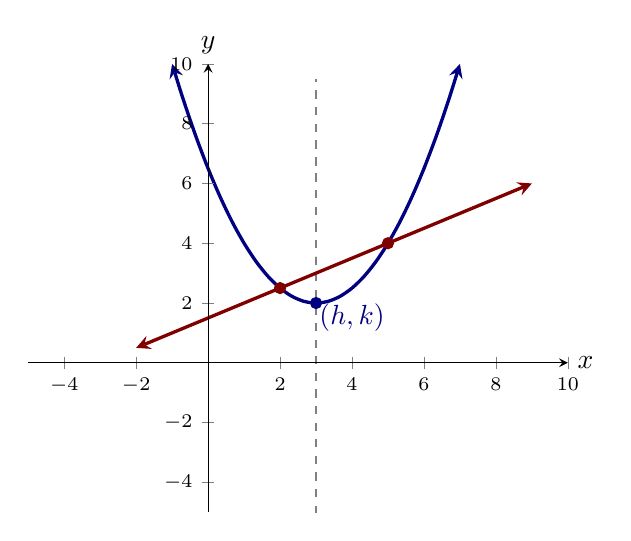
\begin{tikzpicture}
     \begin{axis}[
                domain=-5:10, ymax=10, xmax=10, ymin=-5, xmin=-5,
                axis lines =center, xlabel=$x$, ylabel=$y$,
                ytick={-4,-2,2,4,6,8,10},
                xtick={-4,-2,2,4,6,8,10},
                ticklabel style={font=\scriptsize},
                every axis y label/.style={at=(current axis.above origin),anchor=south},
                every axis x label/.style={at=(current axis.right of origin),anchor=west},
                axis on top,
                ]


        \addplot [draw=penColor, very thick, smooth, domain=(-1:7),<->] {0.5*(x-3)^2 + 2};
        \addplot [line width=1, gray, dashed,samples=100,domain=(-9.5:9.5)] ({3},{x});
        

        \addplot [color=penColor2,only marks,mark=*] coordinates{(5,4)};
        \addplot [color=penColor2,only marks,mark=*] coordinates{(2,2.5)};
        
        \addplot [draw=penColor2, very thick, smooth, domain=(-2:9),<->] {0.5*(x-5) + 4};

        \addplot [color=penColor,only marks,mark=*] coordinates{(3,2)};
        \node[penColor] at (axis cs:4,1.5) {$(h, k)$};
        %\node[penColor] at (axis cs:5,-9) {$-0.5 x^2 - 5 x + 15.5$};



    \end{axis}
\end{tikzpicture}
\end{image}

Intervals and secants are algebraic and geometric partners. Secants give a picture of rates of change over intervals.



What if we push the secant over a little bit until it becomes a tangent line?







\begin{image}
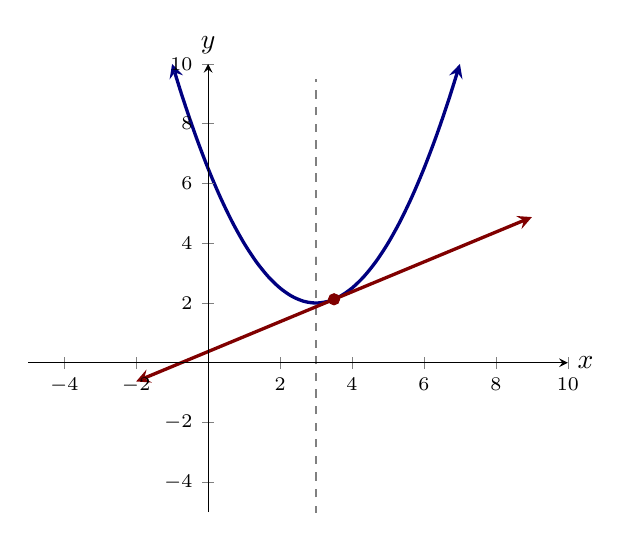
\begin{tikzpicture}
     \begin{axis}[
                domain=-5:10, ymax=10, xmax=10, ymin=-5, xmin=-5,
                axis lines =center, xlabel=$x$, ylabel=$y$,
                ytick={-4,-2,2,4,6,8,10},
                xtick={-4,-2,2,4,6,8,10},
                ticklabel style={font=\scriptsize},
                every axis y label/.style={at=(current axis.above origin),anchor=south},
                every axis x label/.style={at=(current axis.right of origin),anchor=west},
                axis on top,
                ]


        \addplot [draw=penColor, very thick, smooth, domain=(-1:7),<->] {0.5*(x-3)^2 + 2};
        \addplot [line width=1, gray, dashed,samples=100,domain=(-9.5:9.5)] ({3},{x});
        

        \addplot [color=penColor2,only marks,mark=*] coordinates{(3.5,2.125)};
        
        \addplot [draw=penColor2, very thick, smooth, domain=(-2:9),<->] {0.5*(x-3.5) + 2.125};

        %\addplot [color=penColor,only marks,mark=*] coordinates{(3,2)};
        %\node[penColor] at (axis cs:4,1.5) {$(h, k)$};
        %\node[penColor] at (axis cs:5,-9) {$-0.5 x^2 - 5 x + 15.5$};



    \end{axis}
\end{tikzpicture}
\end{image}

Now it is a picture of the rate of change over the interval $\left[ \tfrac{7}{2}, \tfrac{7}{2} \right]$. \\


How should we interpret this? \\


What is the rate of change \textbf{\textcolor{red!90!darkgray}{AT}} a point? \\






\begin{idea}

You cannot calculate the rate of change over an interval with $0$ length.  \\

Therefore, we are inventing an interpretation for the rate of change at a point. \\

We are calling our invention the \textit{instantaneous rate of change}.


\end{idea}











\subsection*{Tangent Lines}

Suppose $f$ is a function.  The graph of $f$ is the collection of points whose coordinates are pairs in $f$.  That is, their coordinates look like $(d, f(d))$.

Suppose $a$ and $b$ are two distinct domain numbers of $f$.  Then the line through $(a, f(a))$ and $(b, f(b))$ is called a secant line.  The slope of this secant line equals the rate of change of $f$ over the interval $[a, b]$.

Tangent lines are degenerate secants. Secant lines need two points on the graph of a function.  A tangent line is a secant line where the two points are the same point. Tangent lines are secant lines created from an interval of length $0$.  But tangent lines are still lines.  They still have a slope.


\textbf{\textcolor{red!90!darkgray}{$\blacktriangleright$}} If the slope of a secant line corresponds to the function's rate of change over an interval, then the slope of a tangent line corresponds to the function's rate of change at a single number.


We are calling this slope of the tangent line the \textbf{\textcolor{purple!85!blue}{instantaneous rate of change}} at the domain number corresponding to the tangent point.




\begin{definition} \textbf{\textcolor{green!50!black}{Instantaneous Rate of Change}}  


Let $f$ be a function. Let $a$ be a number in the domain of $f$.

If the graph of $y = f(x)$ has a non-vertical tangent line at the point $(a, f(a))$, then the slope of this tangent line is the \textbf{instantaneous rate of change} of $f$ \textbf{at} a.


\end{definition}














\subsection*{Quadratics}

We'll begin our investigation into instantaneous rate of change with quadratic functions, whose graphs are parabolas (which never have vertical tangent lines). \\


We need a method of obtaining the slope of tangent lines to parabolas.







$\blacktriangleright$ \textbf{Basic Quadratic}


We'll begin with our basic quadratic function: \textbf{\textcolor{purple!85!blue}{$Q(x) = x^2$}} and its graph \textbf{\textcolor{purple!85!blue}{$y = x^2$}}. \\


We are investigating the graph of $y = x^2$, which is a parabola whose vertex is $(0, 0)$. \\

Let's select a domain number of $Q$, call it $x_0$.   This corresponds to the point $(x_0, y_0) = (x_0, (x_0)^2)$ on the graph of $Q$.

Let's add a picture of the tangent line at $(x_0, y_0) = (x_0, (x_0)^2)$ to our graph of $Q$.


\begin{image}
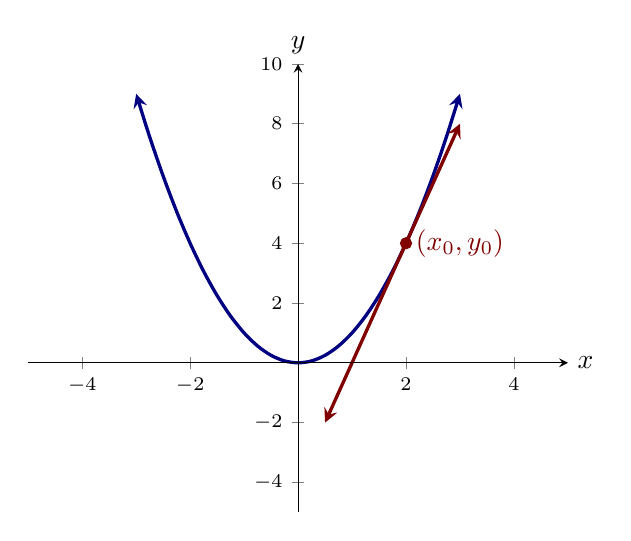
\begin{tikzpicture}
     \begin{axis}[
                domain=-5:5, ymax=10, xmax=5, ymin=-5, xmin=-5,
                axis lines =center, xlabel=$x$, ylabel=$y$,
                ytick={-4,-2,2,4,6,8,10},
                xtick={-4,-2,2,4,6,8,10},
                ticklabel style={font=\scriptsize},
                every axis y label/.style={at=(current axis.above origin),anchor=south},
                every axis x label/.style={at=(current axis.right of origin),anchor=west},
                axis on top,
                ]


        \addplot [draw=penColor, very thick, smooth, domain=(-3:3),<->] {x^2};
        %\addplot [line width=1, gray, dashed,samples=100,domain=(-5:9.5)] ({0},{x});
        

        \addplot [color=penColor2,only marks,mark=*] coordinates{(2,4)};
        \node[penColor2] at (axis cs:3,4) {$(x_0, y_0)$};
        \addplot [draw=penColor2, very thick, smooth, domain=(0.5:3),<->] {4*x - 4};
        


        %\addplot [color=penColor,only marks,mark=*] coordinates{(3,2)};
        %\node[penColor] at (axis cs:2,1.5) {$(h, k)$};




    \end{axis}
\end{tikzpicture}
\end{image}

The tangent line is the graph of a linear function. Let's call this linear function $T$.


$T$ is a linear function. Therefore, the formula for $T$, would look like $T(x) = m(x - x_0) + y_0$, for some $m$.  According to our definition, $m$ is the instantaneous rate of change of $Q$ at $x_0$.  How do we determine its exact value?



\textbf{\textcolor{blue!55!black}{$\blacktriangleright$ We would like a way to obtain the exact value of $m$.}} \\


To get the exact value of $m$, we are going to create a new quadratic function, which will be the difference between the original quadratic function and the linear function.



\begin{explanation}


\[
Q_{new}(x) = Q(x) - T(x) 
\]

\[
Q_{new}(x) = Q(x) - T(x) = x^2 - (m(x - x_0) + y_0)
\]




$Q_{new}(x)$ is a quadratic function and $Q_{new}(x_0) = Q(x_0) - T(x_0) = y_0 - y_0 = 0$. \\


We can also see from the graph above that $Q(x) \geq T(x)$, which means $Q_{new}(x) \geq 0$\\


So, the graph of $Q_{new}(x)$ is a parabola with vertex, $(x_0, 0)$, on the $x$-axis.  The graph of $y = Q(x)$ has slid to the left a distance of $x_0$.  \\


Therefore, the vertex form of $Q_{new}(x)$ is $Q_{new}(x) = (x - x_0)^2 = (x - x_0)(x - x_0)$  \\






\[
Q_{new}(x) = Q(x) - T(x) = x^2 - (m \, (x - x_0) + y_0) 
\]



On the other hand,


\[
Q_{new}(x) = (x - x_0)^2
\]



Therefore, we have

\[
x^2 - (m \, (x - x_0) + y_0) =  (x - x_0)^2
\]


or


\[
x^2 - (m \, (x - x_0) + y_0) =  x^2 - 2 x_0 \, x + x_0^2
\]


or


\[
 -m \, x + m \, x_0 - y_0 =   - 2 \, x_0 \, x + x_0^2
\]


For this to happen, we must have $-m \, x = - 2 \, x_0 \, x$ or \textbf{$m = 2 \, x_0$}. \\


\end{explanation}


At any point $(x_0, y_0)$ on the graph of $y = x^2$, the slope of the tangent line is $2 \, x_0$.  The slope of the tangent line is always twice the $x$-coordinate of the tangent point.




\begin{conclusion} \textbf{\textcolor{green!50!black}{Slope of a Tangent Line}} 


The graph of $y = x^2$ is a parabola.

Let $(x_0, y_0)$ be a point on this parabola.

Then the slope of the tangent line to the parabola at $(x_0, y_0)$ is given by 



\[ \text{slope } \, = \, 2 \, x_0  \]


\end{conclusion}
This for any point on the parabola. \\

What about other parabolas, besides the basic parabola? \\

All parabolas can be obtained from the basic parabola by stretching and shifting. \\



























\subsection*{Stretching}



We can vertically stretch our basic quadratic parabola by multiplying all of the $y$-coordinates by a nonzero constant, $a \ne 0$. \\


The new parabola has an equation of the form $y = a \, x^2$. \\

These are graphs of quadratic functions of the form $Q(x) = a \, x^2$. \\


Let's go through the same process. \\


\begin{explanation}

The tangent line at $(x_0, y_0)$ is the graph of a linear function. Let's call this linear function $T$.


$T$ is a linear function. Therefore, the formula for $T$, would look like $T(x) = m(x - x_0) + y_0$, for some $m$.  According to our definition, $m$ is the instantaneous rate of change of $Q$ at $x_0$.  How do we determine its exact value?


$\blacktriangleright$ We would like a way to obtain the exact value of $m$. \\



To get the exact value of $m$, we are going to create a new quadratic function.



\[
Q_{new}(x) = Q(x) - T(x) = a \, x^2 - (m \, (x - x_0) + y_0)
\]



$Q_{new}(x)$ is a quadratic function and $Q_{new}(x_0) = Q(x_0) - T(x_0) = y_0 - y_0 = 0$. \\

We can also see from the graph that $Q(x) > T(x)$ when $x \ne x_0$, which means $Q_{new}(x) \geq 0$.\\


So, its graph is a parabola with vertex, $(x_0, 0)$, on the $x$-axis.  \\


Therefore, the vertex form of $Q_{new}(x)$ is $Q_{new}(x) = a \, (x - x_0)^2 = (x - x_0)(x - x_0)$  \\






\[
Q_{new}(x) = Q(x) - T(x) = a \, x^2 - (m \, (x - x_0) + y_0) = a \, (x - x_0)^2
\]




\[
a \, x^2 - (m \, (x - x_0) + y_0) = a \, (x - x_0)^2 = a \, x^2 - 2 \, a \, x_0 x + a \, x_0^2
\]



\[
 -m \, x + m \, x_0 - y_0 =   - 2 \, a \, x_0 \, x + a \, x_0^2
\]


For this to happen, we must have $-m \, x = - 2 \, a \, x_0 \, x$ or \textbf{$m = 2 \, a \, x_0$}. \\


\end{explanation}

At any point $(x_0, y_0)$ on the graph of $y = a \, x^2$, the slope of the tangent line is $2 \, a \, x_0$.  The slope of the tangent line is always $2a$ times the $x$-coordinate of the tangent point.










\begin{conclusion} \textbf{\textcolor{green!50!black}{Slope of a Tangent Line}} 


The graph of $y = a \, x^2$ is a parabola.

Let $(x_0, y_0)$ be a point on this parabola.

Then the slope of the tangent line to the parabola at $(x_0, y_0)$ is given by 



\[ \text{slope } \, = \, 2 \, a \, x_0  \]


\end{conclusion}
This for any point on the parabola.




















\subsection*{Shifting}




Beginning with $Q(x) = a \, x^2$ and its parabola $y = a \, x^2$, we can shift horizontally and vertically. \\





Shifting keeps the shape of the parabola, $y = a \, x^2$, intact. \\


The new shifted parabola has an equation of the form $y = a \, (x - h)^2 + k$.

These are graphs of quadratic functions of the form $Q_{new}(x) = a \, (x - h)^2 + k$. \\


If we pick any point, $(x_0, y_0)$, on this parabola, then the slope of the tangent line is the same as the slope of the tangent line for $y = a \, x^2$ at the point $(x_0 - h, y_0 - k)$, because the actual shape of the parabola is not changed by shifting.  \\

From above, we know this slope is \textbf{$2 \, a \, (x_0 - h)$}.






\begin{conclusion} \textbf{\textcolor{green!50!black}{Slope of a Tangent Line}} 


The graph of $y = a \, (x - h)^2 + k$ is a parabola.

Let $(x_0, y_0)$ be any point on this parabola.

Then the slope of the tangent line to the parabola at $(x_0, y_0)$ is given by 



\[ \text{slope } \, = \, 2 \, a \, (x_0 - h)  \]


\end{conclusion}


Every parabola can be described by an equation of the form $y = a \, (x - h)^2 + k$. \\

Our slope of tangent line idea can be applied to every parabola. \\

We have covered every parabola. \\














\begin{theorem} \textbf{\textcolor{green!50!black}{Slope of a Tangent Line (Parabola)}} 


The graph of $y = a (x - h)^2 + k$ is a parabola.

Let $(x_0, y_0)$ be any point on this parabola.

Then the slope of the tangent line to the parabola at $(x_0, y_0)$ is given by 



\[ 2 \, a \, (x_0 - h) \]


\end{theorem}












\textbf{Note:} If we look at the vertex of the parabola $(x_0, y_0) = (h, k)$, then $2 a (x_0 - h) = 2 a (h - h) = 0$ and the slope of the tangent line is $0$, just like we had reasoned before. \\











\section*{iRoC}

Let $Q(x) = a (x - h)^2 + k$ be any quadratic function.

Every point, $(x_0, y_0)$, on the graph of $y = Q(x)$ has a tangent line.

Each tangent line has a slope, which we are calling the instantaneous rate of change of $Q$ at $x_0$.


\textbf{\textcolor{red!90!darkgray}{$\blacktriangleright$}} We can create a new function from this.



\begin{definition} \textbf{\textcolor{green!50!black}{iRoC}}  


Given a quadratic function, $Q(x) = a (x - h)^2 + k$, we define \textbf{the instantaneous rate of change of Q} to be the slope of the tangent line on the graph of $y = Q(x)$ at the point $(x, y)$.


The function $iRoC_Q(x)$ is defined to equal the slope of the tangent line at the point $(x, y)$.


$iRoC_Q(x)$ is a linear function given by 

\[  iRoC_Q(x) = 2 a (x-h) \]

\end{definition}


We now have a function, with a formula, for measuring the instantaneous rate of change of any quadratic function at any domain number. \\


\textbf{\textcolor{red!90!darkgray}{$\blacktriangleright$}} The instantaneous rate of change of the quadratic function, $Q(x) = a \, (x - h)^2 + k$, is the linear function, $iRoC_Q(x) = 2 \, a \, (x-h)$. \\




We can add this to our growing collection. \\ 


\textbf{\textcolor{red!90!darkgray}{$\blacktriangleright$}} The instantaneous rate of change of the linear function, $L(x) = m \, x + b$, is the constant function, $iRoC_L(x) = m$. \\



\textbf{\textcolor{red!90!darkgray}{$\blacktriangleright$}} The instantaneous rate of change of the constant function, $C(x) = c$, is the zero function, $iRoC_C(x) = 0$. \\





\begin{notation} \textbf{\textcolor{blue!55!black}{Language}} 


We are just beginning our investigation of function behavior, so we have given our new function a very descriptive name, \textbf{\textcolor{blue!55!black}{Instantaneous Rate of Change}},  \textbf{\textcolor{blue!55!black}{$iRoC$}}. \\


Calculus uses the name \textbf{\textcolor{blue!55!black}{Derivative}} and it uses a little prime sign as the notation.



\[
iRoC_f(x) = f'(x)
\]


People pronounce $f'(x)$ as ``f prime of $x$''.


\end{notation}

We will use both names.  This will keep the idea fresh in our heads and also give us experience with Calculus notation.






\begin{notation} \textbf{\textcolor{red!70!black}{A Peek Ahead}}


We are beginning our investigation of function analysis at the beginning.  Our formulas have one variable.  But, later, in Calculus, it may not be so clear on what the variable is or what the function is. \\

For this reason, Calculus introduces more notation that is very explicit on this matter.



\[
iRoC_f(x) = f'(x) = \frac{df}{dx}
\]


People pronounce $\frac{df}{dx}$ as ``dfdx''.  They just say the letters.


\end{notation}









\begin{center}
\textbf{\textcolor{green!50!black}{ooooo-=-=-=-ooOoo-=-=-=-ooooo}} \\

more examples can be found by following this link\\ \link[More Examples of Quadratic Behavior]{https://ximera.osu.edu/csccmathematics/precalculus1/precalculus1/quadraticBehavior/examples/exampleList}

\end{center}






\end{document}




